\subsection{Learning Statistics}

\subsubsection{Training Progress}

Figure (\ref{fig:training_loss}) shows the policy objective (eq. \ref{eq:total_objective_function}) over the 3000 training iterations for the DICE 2016 and DICE 2023 versions of ACE. In both versions, the objective falls by several orders of magnitude within the first few iterations, as the network moves from its random initialization to controls and costates of the right magnitude. The initial value is much larger for the 2023 version (about \(2 \cdot 10^{9}\) against \(44\) for the 2016 version), because the randomly initialized network produces an extreme first episode, but this has no lasting effect on training.

After the initial drop, the objective decreases steadily throughout training, from around \(10^{-2}\) after 300 iterations to \(6.3 \cdot 10^{-6}\) for the 2016 version and \(4.1 \cdot 10^{-5}\) for the 2023 version in the final iteration. The fluctuations visible in the middle of training shrink as the cosine schedule lowers the learning rate, and neither run shows the large spikes or exploding gradients observed with the original implementation. The lowest objective on a full episode, which determines the weights used for the results, is \(6.0 \cdot 10^{-6}\) for the 2016 version and \(2.9 \cdot 10^{-5}\) for the 2023 version.

\begin{figure}[ht]
  \centering
  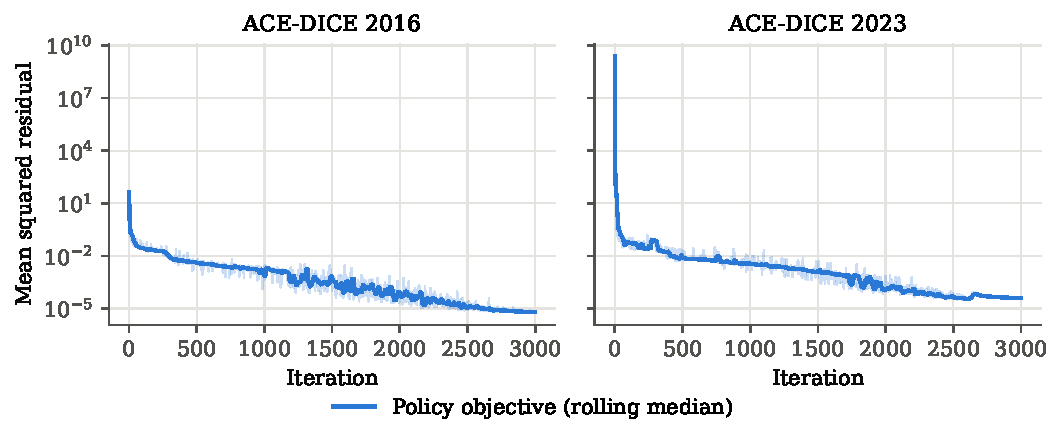
\includegraphics[width=1.0\textwidth]{images/ch6/revised/training_loss.pdf}
  \caption{Policy objective over training iterations (light line: per iteration; dark line: rolling median over 25 iterations)}
  \label{fig:training_loss}
\end{figure}

\subsubsection{Errors in Equilibrium Conditions}

The errors in the individual components that make up the total objective function, as given in equation (\ref{eq:total_objective_function}), are presented in Tables (\ref{table:errors2016}) and (\ref{table:errors-2023}), and summarized in Figure (\ref{fig:residuals}). The statistics in each column are the absolute errors \(|\ell_m|\) of the respective condition over an episode of 128 periods simulated with the best-performing network. The residuals are measured in the scaled units of section (\ref{subsubsec:objective_scaling}), so a residual of \(10^{-3}\) in \(\ell_1\) corresponds to an error of about \(10^{-3} \cdot c_M = 10^{-7}\) in the carbon costates, or about 0.1\% of their value.

\begin{table}[ht]
\centering
\begin{adjustbox}{width=\textwidth,center}
\begin{tabular}{lrrrrrrrrrrr}
\toprule
Statistic & $\ell_0$ & $\ell_{1,M_1}$ & $\ell_{1,M_2}$ & $\ell_{1,M_3}$ & $\ell_{2,\tau_1}$ & $\ell_{2,\tau_2}$ & $\ell_3$ & $\ell_4$ & $\ell_{5,A}$ & $\ell_{5,B}$ & $\ell_6$ \\
\midrule
mean & 2.4e-04 & 3.2e-04 & 1.4e-04 & 1.9e-05 & 2.3e-04 & 4.6e-05 & 2.4e-04 & 7.9e-04 & 4.4e-04 & 1.9e-04 & 7.9e-04 \\
std & 2.1e-04 & 2.6e-04 & 9.1e-05 & 1.3e-05 & 2.0e-04 & 4.4e-05 & 2.0e-04 & 7.8e-04 & 1.6e-03 & 1.7e-04 & 8.0e-04 \\
min & 9.8e-07 & 1.5e-06 & 2.0e-07 & 6.5e-07 & 4.5e-07 & 3.7e-08 & 2.5e-06 & 4.1e-06 & 9.5e-07 & 1.2e-06 & 7.6e-06 \\
25\% & 8.8e-05 & 1.3e-04 & 6.9e-05 & 9.2e-06 & 9.4e-05 & 1.7e-05 & 1.0e-04 & 2.8e-04 & 9.5e-07 & 5.9e-05 & 2.3e-04 \\
50\% & 1.9e-04 & 2.8e-04 & 1.4e-04 & 1.7e-05 & 1.8e-04 & 3.8e-05 & 2.1e-04 & 5.8e-04 & 1.1e-06 & 1.2e-04 & 5.6e-04 \\
75\% & 3.4e-04 & 4.1e-04 & 2.0e-04 & 2.8e-05 & 2.9e-04 & 5.5e-05 & 2.9e-04 & 1.0e-03 & 1.6e-04 & 2.9e-04 & 1.1e-03 \\
99.9\% & 1.2e-03 & 1.3e-03 & 5.1e-04 & 7.2e-05 & 1.1e-03 & 2.8e-04 & 9.2e-04 & 4.1e-03 & 1.4e-02 & 8.3e-04 & 4.0e-03 \\
max & 1.2e-03 & 1.3e-03 & 5.1e-04 & 7.5e-05 & 1.1e-03 & 2.8e-04 & 9.2e-04 & 4.1e-03 & 1.4e-02 & 8.3e-04 & 4.0e-03 \\
\bottomrule
\end{tabular}

\end{adjustbox}
\caption{Error Statistics ACE-DICE (2016 DICE), absolute errors \(|\ell_m|\)}
\label{table:errors2016}
\end{table}

\begin{table}[ht]
\centering
\begin{adjustbox}{width=\textwidth,center}
\begin{tabular}{lrrrrrrrrrrr}
\toprule
Statistic & $\ell_0$ & $\ell_{1,M_1}$ & $\ell_{1,M_2}$ & $\ell_{1,M_3}$ & $\ell_{2,\tau_1}$ & $\ell_{2,\tau_2}$ & $\ell_3$ & $\ell_4$ & $\ell_{5,A}$ & $\ell_{5,B}$ & $\ell_6$ \\
\midrule
mean & 1.7e-03 & 1.3e-03 & 4.4e-04 & 1.5e-05 & 8.1e-04 & 1.4e-04 & 1.4e-03 & 1.2e-03 & 8.6e-04 & 4.9e-04 & 2.3e-03 \\
std & 1.4e-03 & 8.9e-04 & 3.5e-04 & 1.3e-05 & 6.6e-04 & 1.3e-04 & 1.1e-03 & 1.4e-03 & 2.8e-03 & 3.8e-04 & 1.9e-03 \\
min & 6.9e-06 & 3.9e-05 & 3.5e-06 & 4.0e-08 & 3.4e-06 & 1.5e-06 & 1.9e-05 & 1.3e-05 & 9.5e-07 & 1.6e-06 & 7.6e-06 \\
25\% & 6.0e-04 & 6.3e-04 & 2.0e-04 & 5.9e-06 & 1.9e-04 & 5.2e-05 & 6.0e-04 & 3.7e-04 & 9.5e-07 & 1.7e-04 & 8.8e-04 \\
50\% & 1.3e-03 & 1.1e-03 & 3.1e-04 & 1.2e-05 & 6.7e-04 & 9.4e-05 & 1.1e-03 & 7.0e-04 & 1.1e-06 & 3.9e-04 & 1.6e-03 \\
75\% & 2.6e-03 & 1.8e-03 & 6.2e-04 & 2.2e-05 & 1.3e-03 & 1.6e-04 & 2.0e-03 & 1.7e-03 & 3.5e-04 & 8.1e-04 & 3.3e-03 \\
99.9\% & 5.8e-03 & 4.1e-03 & 1.7e-03 & 7.0e-05 & 2.8e-03 & 5.1e-04 & 5.2e-03 & 9.0e-03 & 2.3e-02 & 1.6e-03 & 8.2e-03 \\
max & 5.8e-03 & 4.1e-03 & 1.7e-03 & 7.1e-05 & 2.8e-03 & 5.1e-04 & 5.3e-03 & 9.3e-03 & 2.4e-02 & 1.7e-03 & 8.2e-03 \\
\bottomrule
\end{tabular}

\end{adjustbox}
\caption{Error Statistics ACE-DICE (2023 DICE), absolute errors \(|\ell_m|\)}
\label{table:errors-2023}
\end{table}

For the 2016 version, the mean absolute errors of all conditions lie between \(2 \cdot 10^{-5}\) and \(8 \cdot 10^{-4}\), and the maximum error over the episode is below \(5 \cdot 10^{-3}\) for every condition except the Fischer-Burmeister function \(\ell_{5,A}\). The largest errors are in the emissions condition \(\ell_4\) and the Bellman equation \(\ell_6\). The errors for the 2023 version are mostly larger, by up to a factor of seven, but the maximum error remains below \(10^{-2}\) for every condition except \(\ell_{5,A}\). For the consumption condition \(\ell_3\) and the Bellman equation \(\ell_6\), which are measured in the same units as in the original implementation, the mean errors are about two orders of magnitude smaller than before. The comparison is only indicative, as the original errors measured residuals of different, partly incorrect, conditions.

The largest errors of \(\ell_{5,A}\) occur at the few periods in which the analytical abatement rate reaches one and the constraint \(E_t \geq 0\) starts to bind, around 2175 for the 2016 version and 2190 for the 2023 version. There, the complementarity condition switches between its two branches, which the smooth policy network can only approximate, and the median error of \(\ell_{5,A}\) is about \(10^{-6}\) in both versions.

\begin{figure}[ht]
  \centering
  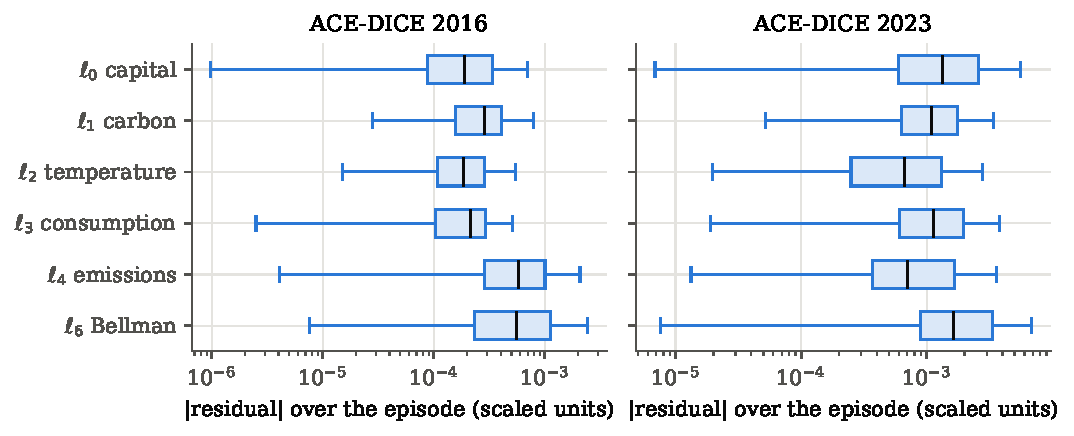
\includegraphics[width=1.0\textwidth]{images/ch6/revised/residuals.pdf}
  \caption{Distribution of the absolute errors over the simulated episode. For conditions with several components, the largest component in each period is shown. Boxes show the interquartile range, whiskers the full range.}
  \label{fig:residuals}
\end{figure}
